% =========================================================
% CONFIGURACION DEL DOCUMENTO
% =========================================================
\providecommand{\main}{..}
\documentclass[\main/main.tex]{subfiles}

% =========================================================
% CONTENIDO
% =========================================================
\begin{document}
\chapter{Resultados}
\label{cha:04_resultados}
    Debido a que este trabajo de título consistió en la construcción de un sistema para configurar y ejecutar experimentos es que se opta por presentar estos resultados a modo de un manual de usuario.

    \section{Configurar un experimento.}
    \label{sec:04_configurar}
        Para configurar y almacenar un experimento se requieren los siguientes módulos:

\begin{singlespace}\begin{python}
import os
from saccadeApp import SaccadeDB
from saccadeApp import Experiment, Test, Frame, Component
\end{python}\end{singlespace}
    
        Donde \pythonInline{os} se utiliza para la manipulación de directorios y archivos, \pythonInline{SaccadeDB} para el manejo de la base de datos y \pythonInline{Experiment, Test, Frame, Component} para configurar todos los elementos asociados a un experimento.

        En primera instancia, es necesario crear el directorio en donde se almacenarán las configuraciones:

\begin{singlespace}\begin{python}
base_dir = u'C:\\Experiments'

if not os.path.isdir(base_dir):
    os.mkdir(base_dir) 
\end{python}\end{singlespace}
        
        Luego, se crea la base de datos en este directorio, para lo cual se utiliza el módulo \pythonInline{SaccadeDB}. Al inicializar un objeto de este tipo debe indicarse la ubicación y nombre del archivo de base de datos a utilizar, si este no existe se creará uno. En caso de no especificar el archivo de base de datos, esta función crea uno en la carpeta donde se encuentra el ejecutable del programa con el nombre por defecto ''saccadedb.sqlite3''.   

\begin{singlespace}\begin{python}
data = SaccadeDB(base_dir + u'\\test_database.sqlite3')
\end{python}\end{singlespace}

        Una vez que la base de datos es creada se hace posible almacenar las configuraciones. El experimento a construir se compondrá de dos tareas que se ejecutarán una sola vez, de forma secuencial, y luego de que el usuario presione la tecla ''espacio''. 

        La primera corresponderá a una tarea asociada a movimiento prosacádico con efecto de \textit{overlap}, lo que implica que el estímulo central se encontrará presente en todos los cuadros. Los componentes a configurar son dos: El estímulo central (cruz de color blanco) y el objetivo (cuadrado de color rojo), que serán ubicados en el centro de la pantalla y $16\degree$ a la derecha, respectivamente. 

\begin{singlespace}\begin{python}
cross = Component()
cross.set_name(u'CP')
cross.set_size(1.0)
cross.set_shape(u'cross')
cross.set_color(u'white')
cross.set_position(0.0, 0.0)

target = Component()
target.set_name(u'TP')
target.set_size(1.0)
target.set_shape(u'square')
target.set_color(u'red')
target.set_position(16.0, 0)
\end{python}\end{singlespace}

        Con los componentes creados, es posible configurar los cuadros a presentar durante la presentación de la tarea. El primer y tercer cuadro solo presentan el estímulo central, mientras que el segundo incluye además el objetivo. Los tiempos de presentación de cada cuadro son $1.8[s]$ para el primer cuadro, $1.5[s]$ para el segundo y $1.0[s]$ para el tercero. 

\begin{singlespace}\begin{python}
frame1 = Frame()
frame1.set_name(u'Central Stimulus')
frame1.set_time(1.8)
frame1.set_as_task(False)
frame1.set_color(u'black')
frame1.component_add(cross)

frame2 = frame1.copy()
frame2.set_name(u'Target')
frame2.set_time(1.5)
frame2.component_add(target)

frame3 = frame1.copy()
frame3.set_time(1.0)
\end{python}\end{singlespace}

        Por último, se crea la tarea asignándole un nombre. Se configura para una sola repetición y se indican los cuadros que considerará. 

\begin{singlespace}\begin{python}
test1 = Test()
test1.set_name(u'Overlap Task')
test1.set_quantity(1)
test1.frame_add(frame1)
test1.frame_add(frame2)
test1.frame_add(frame3)
\end{python}\end{singlespace}

        La segunda tarea a configurar corresponde a una única imagen centrada. En este caso, el cuadro fue configurado para no depender del tiempo pero si de la entrada de teclado realizada por el usuario.  

\begin{singlespace}\begin{python}
image = Component()
image.set_image(u'image.png')

frame4 = Frame()
frame4.set_name(u'Image Presentation')
frame4.set_as_task(True)
frame4.set_keys_allowed(u'space')
frame4.set_keys_selected(u'space')
frame4.component_add(image)

test2 = Test()
test2.set_name(u'Search task')
test2.set_quantity(1)
test2.frame_add(frame4)
\end{python}\end{singlespace}

        Para crear y almacenar un experimento es necesario indicar la base de datos en donde se almacenarán las configuraciones. De forma posterior, es necesario identificar al experimento otorgándole tanto un código único como un nombre, además de la versión a la cual corresponde. Se recomienda realizar las configuraciones y añadir tareas luego de esto.

        Para hacer evidente durante la ejecución de este ejemplo el momento en que inicia cada una de las tareas, se configura que el usuario deba presionar la tecla ''espacio'' cuando una comience. Finalmente y por simplicidad, se evita que aparezca el diálogo para ingresar características del usuario. 

\begin{singlespace}\begin{python}
experiment = Experiment()
experiment.set_database(data)

experiment.set_code(u'expcode_01')
experiment.set_info(u'Experiment test', u'v1.0')
experiment.set_space_start(True)
experiment.set_dialog(status=False)
experiment.test_add(test1)
experiment.test_add(test2)
experiment.save()
\end{python}\end{singlespace}

    \section{Ejecutar un experimento.}
    \label{sec:04_ejecutar}
        Para ejecutar un experimento es necesario que este se encuentre almacenado en la base de datos y que exista además un perfil de configuración que indique tanto el monitor, \textit{eye tracker} y directorio de resultados a utizar. A continuación se indican los módulos necesarios para crear dicho perfil y ejecutar el experimento almacenado en el punto anterior: 

\begin{singlespace}\begin{python}
import os
from saccadeApp import SaccadeDB
from saccadeApp import Master
from saccadeApp import ExperimentHandler
\end{python}\end{singlespace}
        
        Donde \pythonInline{os} se utiliza para la manipulación de directorios y archivos, \pythonInline{SaccadeDB} para el manejo de la base de datos, \pythonInline{Master} para la configuración del hardware a utilizar y setear la carpeta donde se almacenarán los resultados y \pythonInline{ExperimentHandler} para ejecutar el experimento seleccionado.

        Para crear el perfil de configuración es necesario: Contar con una base de datos disponible, crear o comprobar que existe el directorio en donde se almacenanarán los resultados del experimento y definir las características del monitor a utilizar en PsychoPy. 

        Como base de datos se utilizará la que fue creada en el punto anterior.

\begin{singlespace}\begin{python}
data = SaccadeDB(base_dir + u'\\test_database.sqlite3')
\end{python}\end{singlespace}

        Por simplicidad y claridad el directorio para los resultados de los experimentos se creará dentro de la carpeta definida en el punto anterior.

\begin{singlespace}\begin{python}
base_dir = u'C:\\Experiments'
data_dir = base_dir + u'\\Events'

if not os.path.isdir(data_dir):
    os.mkdir(data_dir) 
\end{python}\end{singlespace}

        Para asegurar que los estímulos presentados por pantalla tengan las dimensiones definidas en la configuración del experimento, es necesario verificar que el monitor a utilizar tenga un perfil de configuración. Dichos perfiles deben ser definidos por medio de la herramienta dispuesta por PsychoPy llamada \textit{''Monitor Center''}\footnote{Centro de monitores.} que puede ser ejecutada directamente desde el script mediante el comando \pythonInline{Master.open_psychopy_monitor_center()}. En ella (ver figura \ref{fig:04_monitor_center}) es posible definir las proporciones físicas del monitor, sus características lumínicas y distancia al usuario. Para efecto de este ejemplo, se creará un perfil llamado ''my\_monitor'' y se ingresarán unicamente los atributos asociados a la distancia al usuario ($53[cm]$), tamaño en pixeles ($1680\times1050[px]$) y ancho efectivo de la pantalla ($47.5[cm]$).
        \begin{figure}[H]
            \centering
            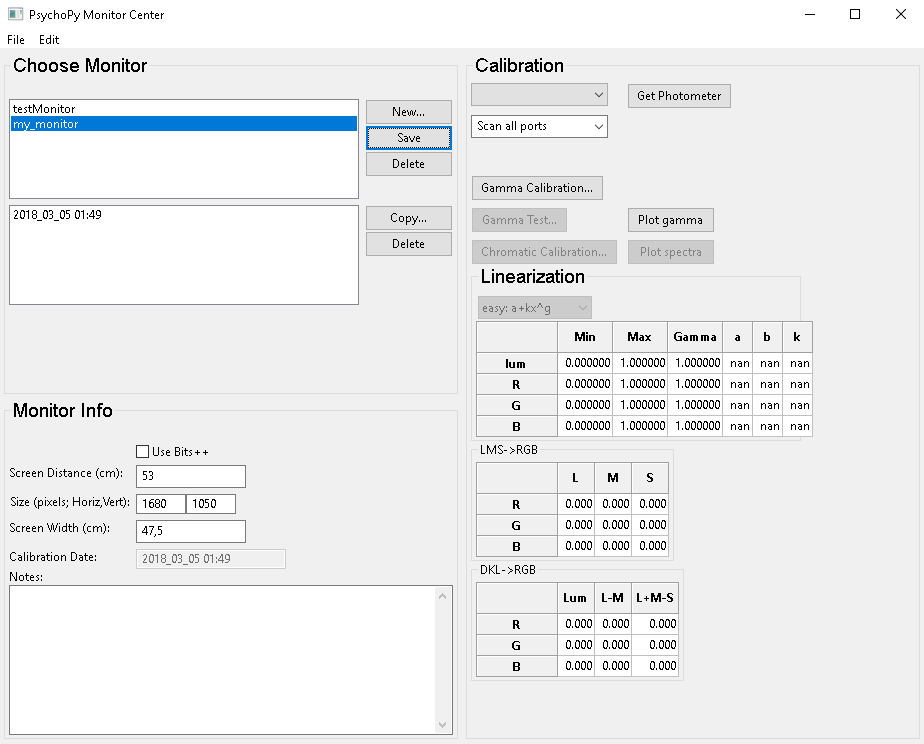
\includegraphics[width=0.6\textwidth]{cap_04_monitorcenter}
            \caption{Centro de monitores de PsychoPy.}
            \label{fig:04_monitor_center}
        \end{figure} 

        Luego, es posible crear el perfil de configuración requerido. Este incluirá el monitor que se acaba de definir, que en este caso corresponde a la pantalla secundaria, el \textit{eye tracker}, que en este caso es un ''eyetribe'' y la carpeta de resultados creada al comienzo. De forma similar al proceso de creación del experimento es necesario indicar en que base de datos será almacenado, en este caso el nombre del perfil de configuración funciona como clave única y por tanto lo identifica.

\begin{singlespace}\begin{python}
conf = Master()
conf.set_database(data)

conf.set_name(u'my_profile')
conf.set_monitor(u'test_monitor')
conf.set_screen(1)
conf.set_tracker(u'eyetribe')
conf.set_experiment_path(data_dir)
conf.save()
\end{python}\end{singlespace}

        Finalmente, el experimento definido el el punto anterior se ejecuta con los siguientes comandos:

\begin{singlespace}\begin{python}
execution = ExperimentHandler()

if execution.load_configuration(db=data, master=u'my_profile', experiment=u'expcode_01'):
    execution.save_parameters()
    execution.execute_experiment()
\end{python}\end{singlespace}  

    \section{Comprobación de funcionamiento.}
    \label{sec:04_resultados}
        Para comprobar de que los datos estuvieran siendo registrados correctamente se creó un experimento cuya tarea principal solo contenía la imagen presentada en la figura \ref{fig:04_frame_result}.a. La tarea consistía en realizar una inspección visual, los resultados se presentan en \ref{fig:04_frame_result}.b.

        \begin{figure}[H]
            \centering
            \subfloat[Imagen original.]{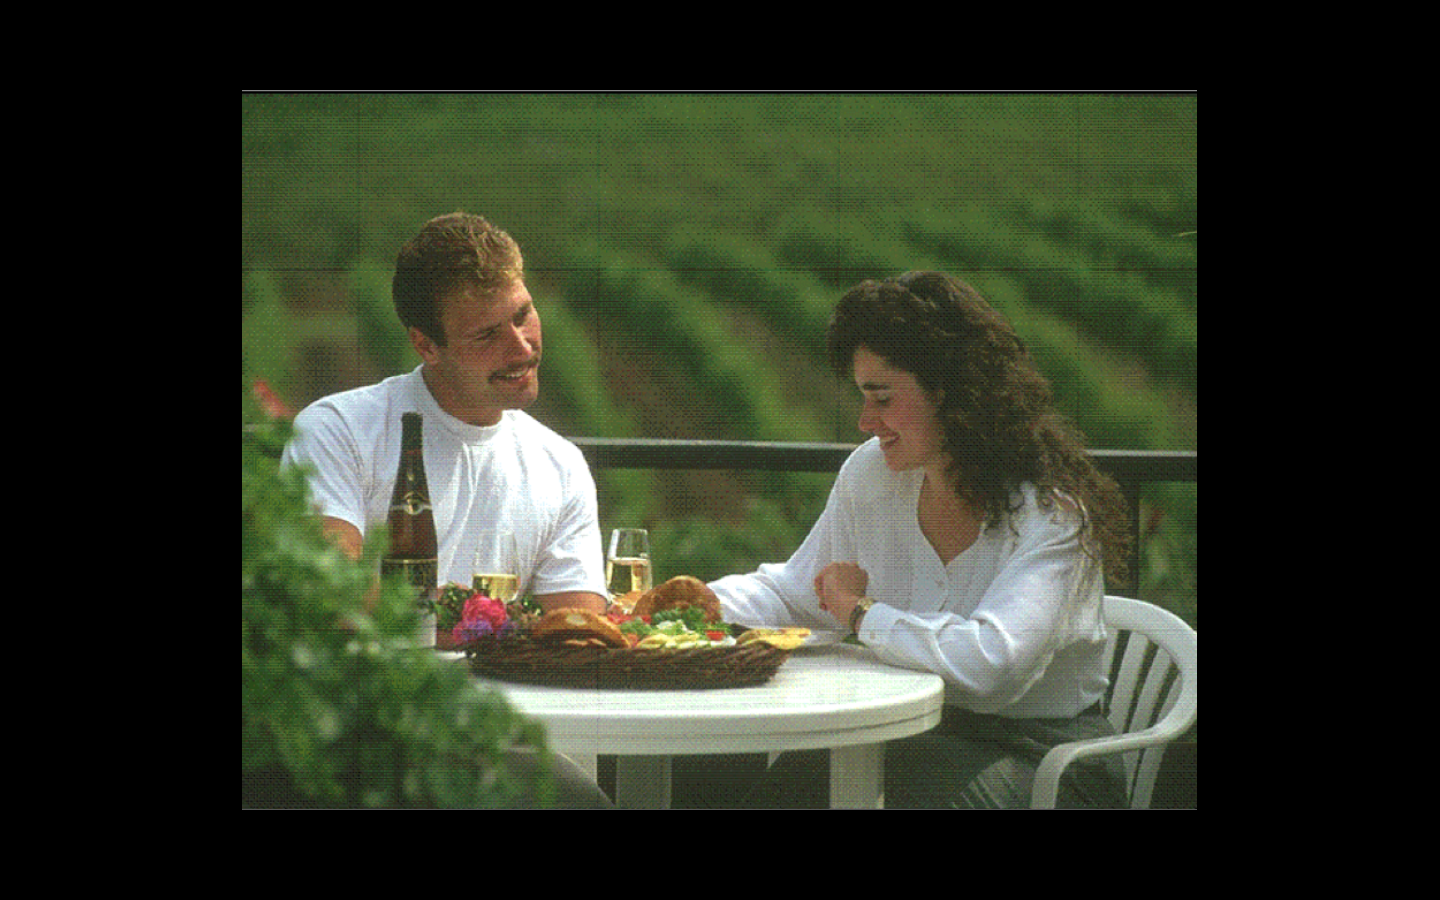
\includegraphics[width=0.45\textwidth]{cap_04_resultado_orig}}\hspace{5mm}
            \subfloat[Movimiento ocular registrado.]{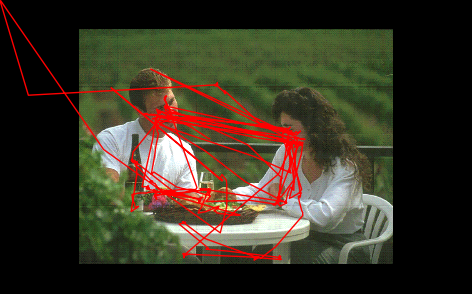
\includegraphics[width=0.45\textwidth]{cap_04_resultado_sist}}
            \caption{Datos registrados.}
            \label{fig:04_frame_result}
        \end{figure}

        Es posible apreciar en los datos registrados que el movimiento ocular en esta imagen se realiza principalmente entre los rostros de la pareja y las proyecciones de hacia donde se encuentran dirigidas sus miradas.

        Al consultar los registros de los puntos ubicados en la esquina superior izquierda y que parecieran no corresponder al patrón de observación se determina que estos corresponden a los momentos en que el usuario cierra los ojos.    
        


	% ===============================================================
	% ===============================================================
\end{document}